\documentclass[tikz,border=10pt]{standalone}
\usepackage{tikz}
\usepackage{pgfplots}
\pgfplotsset{compat=1.18}

\begin{document}

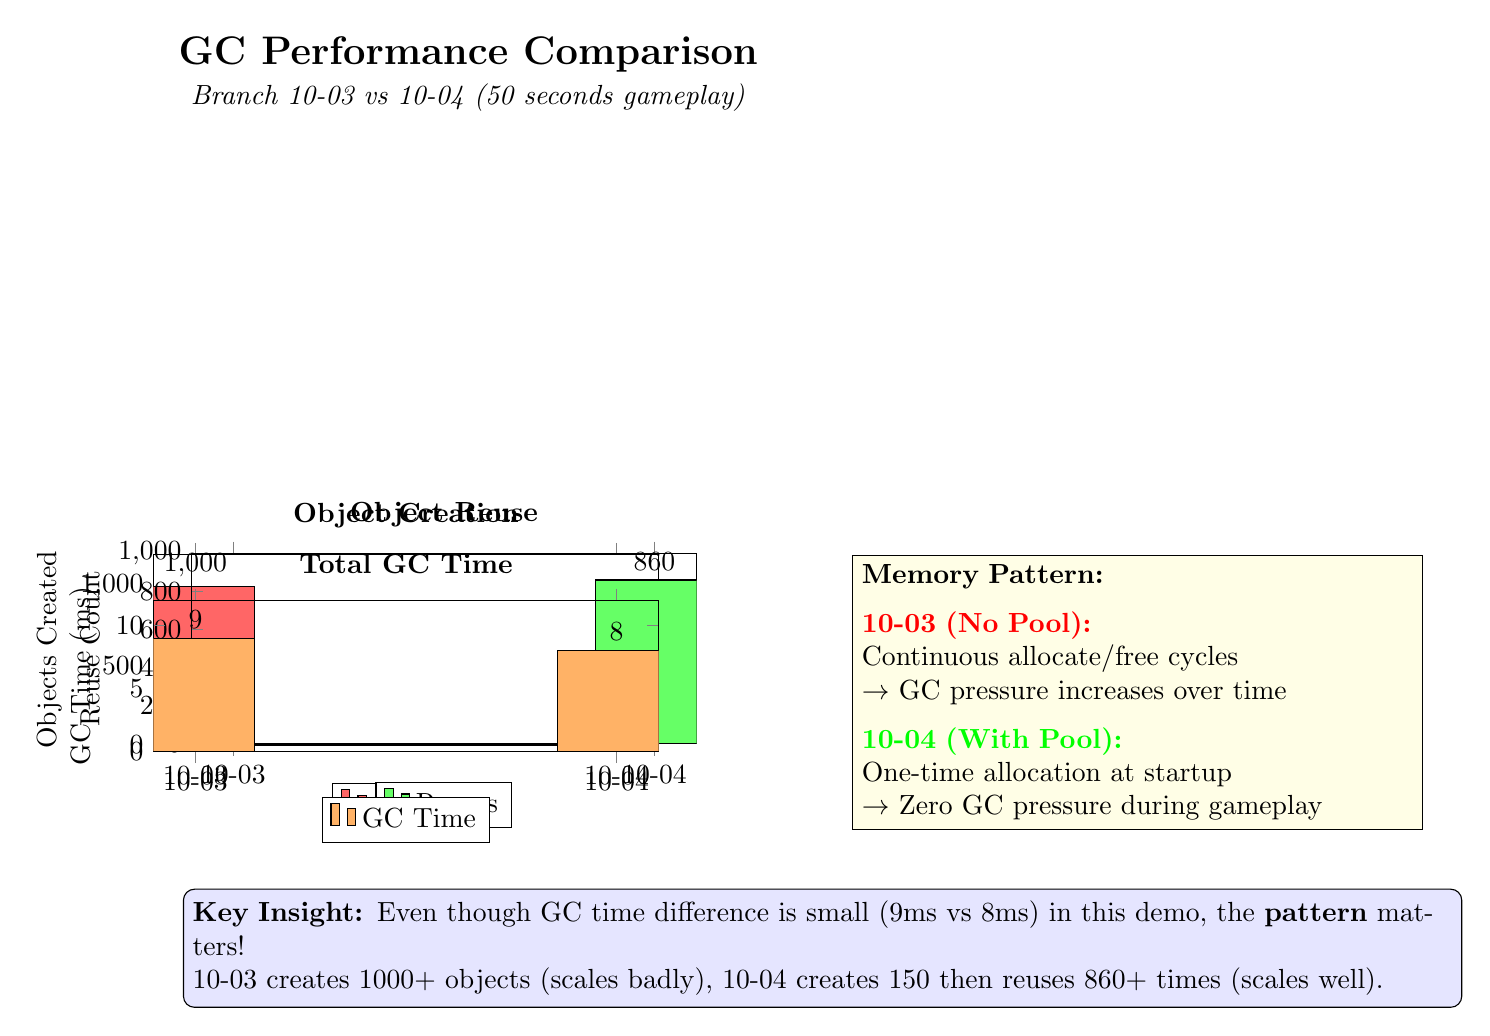
\begin{tikzpicture}
    % Title
    \node [above] at (4,8.5) {\Large\textbf{GC Performance Comparison}};
    \node [above] at (4,8) {\textit{Branch 10-03 vs 10-04 (50 seconds gameplay)}};

    % Bar chart: Objects created
    \begin{axis}[
        name=objects,
        at={(0,4)},
        ybar,
        bar width=1.5cm,
        width=8cm,
        height=4cm,
        ylabel={Objects Created},
        symbolic x coords={10-03, 10-04},
        xtick=data,
        nodes near coords,
        nodes near coords align={vertical},
        ymin=0,
        ymax=1200,
        legend style={at={(0.5,-0.2)},anchor=north},
        title={\textbf{Object Creation}},
        ]
        \addplot[fill=red!60] coordinates {(10-03,1000) (10-04,150)};
        \legend{Objects}
    \end{axis}

    % Bar chart: Objects reused
    \begin{axis}[
        name=reuse,
        at={(9,4)},
        ybar,
        bar width=1.5cm,
        width=8cm,
        height=4cm,
        ylabel={Reuse Count},
        symbolic x coords={10-03, 10-04},
        xtick=data,
        nodes near coords,
        nodes near coords align={vertical},
        ymin=0,
        ymax=1000,
        legend style={at={(0.5,-0.2)},anchor=north},
        title={\textbf{Object Reuse}},
        ]
        \addplot[fill=green!60] coordinates {(10-03,0) (10-04,860)};
        \legend{Reuses}
    \end{axis}

    % GC Time comparison
    \begin{axis}[
        name=gc,
        at={(0,0)},
        ybar,
        bar width=1.5cm,
        width=8cm,
        height=3.5cm,
        ylabel={GC Time (ms)},
        symbolic x coords={10-03, 10-04},
        xtick=data,
        nodes near coords,
        nodes near coords align={vertical},
        ymin=0,
        ymax=12,
        legend style={at={(0.5,-0.3)},anchor=north},
        title={\textbf{Total GC Time}},
        ]
        \addplot[fill=orange!60] coordinates {(10-03,9) (10-04,8)};
        \legend{GC Time}
    \end{axis}

    % Memory pattern diagram
    \node [draw, fill=yellow!10, text width=7cm, minimum height=3cm] at (12.5,0.75) {
        \textbf{Memory Pattern:}\\[0.2cm]
        \textcolor{red}{\textbf{10-03 (No Pool):}}\\
        Continuous allocate/free cycles\\
        $\rightarrow$ GC pressure increases over time\\[0.2cm]
        \textcolor{green}{\textbf{10-04 (With Pool):}}\\
        One-time allocation at startup\\
        $\rightarrow$ Zero GC pressure during gameplay
    };

    % Key insight
    \node [draw, fill=blue!10, rounded corners, text width=16cm, minimum height=1.5cm] at (8.5,-2.5) {
        \textbf{Key Insight:} Even though GC time difference is small (9ms vs 8ms) in this demo, the \textbf{pattern} matters!\\
        10-03 creates 1000+ objects (scales badly), 10-04 creates 150 then reuses 860+ times (scales well).
    };

\end{tikzpicture}

\end{document}
